\documentclass[tikz,border=6pt]{standalone}
\usepackage[T1]{fontenc}
\usepackage[utf8]{inputenc}
\usepackage{pgfplots}
\usepgfplotslibrary{groupplots}
\usetikzlibrary{calc}
\pgfplotsset{compat=1.18}
\begin{document}
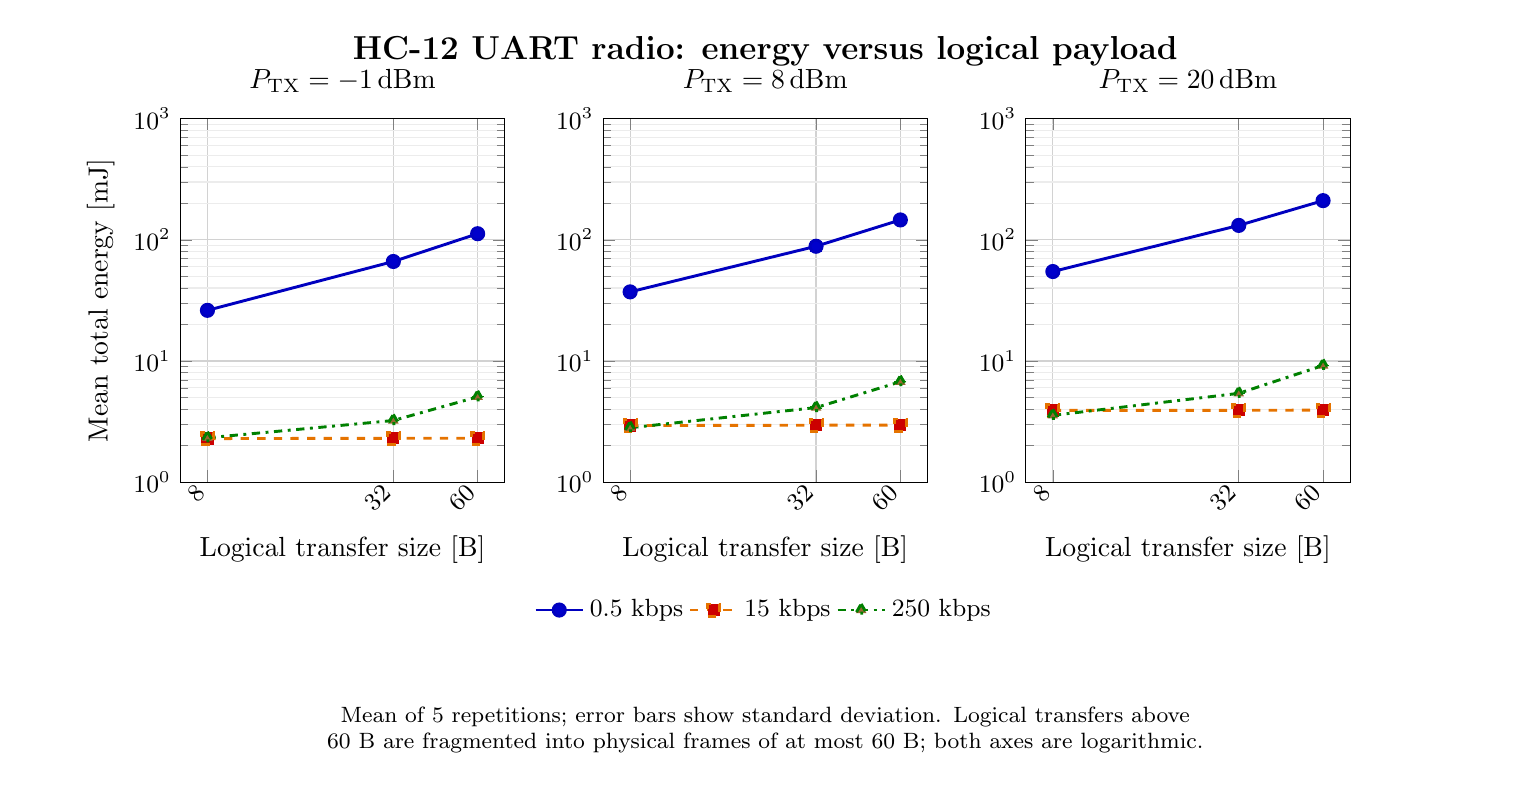
\begin{tikzpicture}
\begin{groupplot}[/pgf/number format/use comma,
  group style={group size=3 by 1, horizontal sep=1.25cm},
  width=5.7cm, height=6.2cm,
  xmode=log, log basis x={2}, ymode=log, log basis y={10},
  ymin=1, ymax=1000,
  xtick={8,32,60}, xticklabels={8,32,60},
  x tick label style={rotate=45, anchor=east, font=\small},
  y tick label style={font=\small},
  grid=both, minor grid style={gray!15}, major grid style={gray!35},
  xlabel={Logical transfer size [B]},
  every axis plot/.append style={line width=1.05pt},
  error bars/error bar style={line width=0.35pt},
  legend style={font=\small, draw=none, fill=none, at={(0.5,-0.29)},
    anchor=north, legend columns=-1},
]
\nextgroupplot[title={\(P_{\mathrm{TX}}=-1\,\mathrm{dBm}\)}, ylabel={Mean total energy [mJ]}]
\addplot+[
  color=blue!75!black, solid, mark=*, mark size=2.2pt,
  error bars/.cd, y dir=both, y explicit,
] coordinates {
  (8,26.1874298) +- (0,0.0270158703)
  (32,66.2334591) +- (0,1.70933688)
  (60,112.267302) +- (0,6.35324089)
};
\addplot+[
  color=orange!90!black, dashed, mark=square*, mark size=2.2pt,
  error bars/.cd, y dir=both, y explicit,
] coordinates {
  (8,2.29170705) +- (0,0.00977897055)
  (32,2.30419208) +- (0,0.00385666479)
  (60,2.30501593) +- (0,0.00535042708)
};
\addplot+[
  color=green!50!black, dashdotted, mark=triangle*, mark size=2.2pt,
  error bars/.cd, y dir=both, y explicit,
] coordinates {
  (8,2.32532944) +- (0,0.0447845324)
  (32,3.23015038) +- (0,0.00252574666)
  (60,5.06168437) +- (0,0.0069044147)
};
\nextgroupplot[title={\(P_{\mathrm{TX}}=8\,\mathrm{dBm}\)}]
\addplot+[
  color=blue!75!black, solid, mark=*, mark size=2.2pt,
  error bars/.cd, y dir=both, y explicit,
] coordinates {
  (8,37.1965248) +- (0,0.890706022)
  (32,88.4658054) +- (0,7.57882451)
  (60,145.832455) +- (0,9.76480473)
};
\addlegendentry{0.5 kbps}
\addplot+[
  color=orange!90!black, dashed, mark=square*, mark size=2.2pt,
  error bars/.cd, y dir=both, y explicit,
] coordinates {
  (8,2.93396178) +- (0,0.00485306335)
  (32,2.95463349) +- (0,0.010462821)
  (60,2.96128362) +- (0,0.0139327486)
};
\addlegendentry{15 kbps}
\addplot+[
  color=green!50!black, dashdotted, mark=triangle*, mark size=2.2pt,
  error bars/.cd, y dir=both, y explicit,
] coordinates {
  (8,2.81565643) +- (0,0.0385046226)
  (32,4.1300426) +- (0,0.0414635597)
  (60,6.74534359) +- (0,0.0135005782)
};
\addlegendentry{250 kbps}
\nextgroupplot[title={\(P_{\mathrm{TX}}=20\,\mathrm{dBm}\)}]
\addplot+[
  color=blue!75!black, solid, mark=*, mark size=2.2pt,
  error bars/.cd, y dir=both, y explicit,
] coordinates {
  (8,54.7319202) +- (0,0.0501987526)
  (32,131.430856) +- (0,5.94934072)
  (60,210.386969) +- (0,11.6108495)
};
\addplot+[
  color=orange!90!black, dashed, mark=square*, mark size=2.2pt,
  error bars/.cd, y dir=both, y explicit,
] coordinates {
  (8,3.91501601) +- (0,0.0119927687)
  (32,3.92126592) +- (0,0.00367067511)
  (60,3.93444517) +- (0,0.0207156758)
};
\addplot+[
  color=green!50!black, dashdotted, mark=triangle*, mark size=2.2pt,
  error bars/.cd, y dir=both, y explicit,
] coordinates {
  (8,3.56210357) +- (0,0.0427165399)
  (32,5.41255194) +- (0,0.018580906)
  (60,9.18572541) +- (0,0.0436861039)
};
\end{groupplot}
\node[font=\bfseries\large] at ($(group c2r1.north)+(0,0.85cm)$)
  {HC-12 UART radio: energy versus logical payload};
\node[font=\footnotesize, align=center, text width=18.5cm]
  at ($(group c2r1.south)+(0,-3.15cm)$)
  {Mean of 5 repetitions; error bars show standard deviation. Logical transfers above 60 B are fragmented into physical frames of at most 60 B; both axes are logarithmic.};
\end{tikzpicture}
\end{document}
